\part{Änderungen des Entwurfs}

\section{DFAFramework}

Die größte Änderung besteht in der Aufteilung des Interfaces \inlinecode{Lattice} in die drei Interfaces \inlinecode{Initializer}, \inlinecode{Transition} und \inlinecode{Join}, jeweils mit dem Typparameter \inlinecode{E extends LatticeElement}, der das verwendete \inlinecode{LatticeElement} angibt.
Dabei hat jedes der drei neuen Interfaces genau eine Methode, die die von dem Interface dargestellte Operation beschreibt:

\begin{itemize}
	\item \inlinecode{Initializer<E extends LatticeElement>}: initialisiert eine Analyse mittels \inlinecode{getInitialStates():Map<Block,BlockState<E> >}
	\item \inlinecode{Join<E extends LatticeElement>}: führt Join-Operationen mittels \inlinecode{join(Set<E>):E} aus
	\item \inlinecode{Transition<E extends LatticeElement>}: führt Transitionen mittels \inlinecode{transition(E,Unit):E} aus
\end{itemize}

Diese Aufteilung ermöglicht eine vollständig modulare Implementierung der Analysen.
\inlinecode{Initializer}, \inlinecode{Join} und \inlinecode{Transition} sind vollständig austauschbar (vorausgesetzt die typparameter sind kompatibel).

Die ehemals abstrakte Klasse \inlinecode{DataFlowAnalysis}\inlinecode{<E extends LatticeElement>} ist nun ein Interface, welches von den Interfaces \inlinecode{Initializer}, \inlinecode{Join} und \inlinecode{Transition} erbt.
Damit stellt \inlinecode{DataFlowAnalysis} alle für die Ausführung einer Datenflussanalyse benötigten Operationen bereit.

Zusätzlich zum Interface \inlinecode{DataFlowAnalysis} wurde noch die abstrakte Klasse \inlinecode{CompositeDataFlowAnalysis}\inlinecode{<E extends LatticeElement>} hinzugefügt, die \inlinecode{DataFlowAnalysis} implementiert und einen Konstruktor bereitstellt, der einen \inlinecode{Initializer}, einen \inlinecode{Join} und eine \inlinecode{Transition} entgegennimmt.
\inlinecode{getInitialStates}, \inlinecode{join} und \inlinecode{transition} werden dann an die entsprechenden Methoden der übergebenen Objekte delegiert.
Dies erlaubt das Zusammensetzten neuer Datenflussanalysen aus einzelnen Komponenten (vorausgesetzt die Typparameter sind kompatibel).

Die Rolle der ehemaligen \inlinecode{DataFlowAnalysis} übernimmt die abstrakte Klasse \inlinecode{DFAFactory<E extends LatticeElement>}.
Damit wurde der Rückgabetyp der Methode \inlinecode{getAnalysis(String)} von \inlinecode{AnalysisLoader} auch zu \inlinecode{DFAFactory} angepasst.

Weiter ist die Klasse \inlinecode{SimpleBlockGraph} hinzugekommen.
Diese erbt von \inlinecode{soot.toolkits.graph.}\inlinecode{BriefBlockGraph} und sorgt lediglich dafür, dass die \inlinecode{getTails}-Methode höchstens einen \inlinecode{Block} zurückgibt (dass es also höchstens einen Endblock gibt). Dies wird durch Einfügen eines künstlichen Endblocks erreicht, falls der ursprüngliche \inlinecode{BriefBlockGraph} mehrere Endblöcke hat.

\newpage
Eine weitere neue Klasse ist \inlinecode{DFAPrecalcController}, welche die Vorberechnung einer \inlinecode{DFAExecution} kontrolliert. Zu diesem Zweck wurde dem Konstruktor ein Parameter vom Typ \inlinecode{DFAPrecalcController} hinzugefügt.
Beispielsweise kann die Vorberechnung mittels \inlinecode{pause(waitTime : int)} pausiert werden und dann mit \inlinecode{continue()} fortgesetzt werden.
Dies ist z. B. nützlich, um zu verhindern, dass zu viel Speicher belegt wird, während sich der Nutzer längere Zeit in einem Menü befindet.
Eine Vorberechnung kann auch mit \inlinecode{stop()} gestoppt werden.
Dann wird ein Zwischenergebnis gespeichert und die Vorberechnung abgebrochen.

Als Exception-Klassen wurden \inlinecode{DFAException} sowie die Unterklassen \inlinecode{UnsupportedValueException} und \inlinecode{UnsupportedStatementException} hinzugefügt.
Diese werden benutzt um Probleme bei der Ausführung einer Datenflussanalyse zu signalisieren (z. B. wenn nicht unterstützte Instruktionen angetroffen werden, die nicht einfach ignoriert werden können).

Schließlich wurde noch das Enum \inlinecode{TaintAnalysisTag} hinzugefügt, welches von \inlinecode{soot.tagkit.AttributeValueException} erbt und benutzt wird, um die \inlinecode{taint}- , \inlinecode{clean}- und \inlinecode{sensitive}-Methoden für die Taint-Analyse zu markieren.

\subsection{Kleine Änderungen}

Im Folgenden werden weitere kleine Änderungen zusammengefasst:

\inlinecode{Color} wurde umbenannt in \inlinecode{LogicalColor}.

Der Parameter \inlinecode{cpy : AnalysisState} im Konstruktor \inlinecode{AnalysisState(..., cpy : AnalysisState)} wurde ersetzt durch die beiden Parameter \inlinecode{stateMap : Map<AbstractBlock, BlockState<E> >} und \inlinecode{colorMap : Map<BasicBlock, LogicalColor>}.
Weiter wurden die \inlinecode{(protected)} Methoden \inlinecode{setStateMap(Map<AbstractBlock,}\inlinecode{BlockState<E>>)}, \inlinecode{getStateMap()}\inlinecode{:Map<AbstractBlock, BlockState<E>>}, \inlinecode{setColorMap(Map<BasicBlock,}\inlinecode{LogicalColor>)}, \inlinecode{getColorMap():Map<BasicBlock,}\inlinecode{LogicalColor>} zum setzen bzw. erhalten der \inlinecode{Map}s für die \inlinecode{BlockState}s und \inlinecode{LogicalColor}s hinzugefügt.
Die Methoden \inlinecode{getState(...):BlockState<E>} und \inlinecode{setState(...)} wurden zu \inlinecode{getBlockState(...):BlockState<E>} und \inlinecode{setBlockState(...)} umbenannt.

In der Klasse \inlinecode{BlockState<E extends LatticeElement>} wurden die beiden \inlinecode{(protected)} Methoden \inlinecode{setInState(E)} und \inlinecode{setOutState(E)} hinzugefügt.

In der Klasse \inlinecode{BasicBlock} wurde die \inlinecode{(protected)} Methode \inlinecode{setElementaryBlocks(List<ElementaryBlock>)} hinzugefügt.
Weiter wurden \inlinecode{setCorrespondingSootBlock(...)} und \inlinecode{getCorrespondingSootBlock()} zu \inlinecode{setSootBlock(...)} und \inlinecode{getSootBlock()} umbenannt.

In der Klasse \inlinecode{ElementaryBlock} wurde die \inlinecode{(protected)} Methode \inlinecode{setUnit(Unit)} hinzugefügt.

\begin{figure}[H]
	\caption{Aktuelles Klassendiagramm für das DFAFramework}
	\centering
	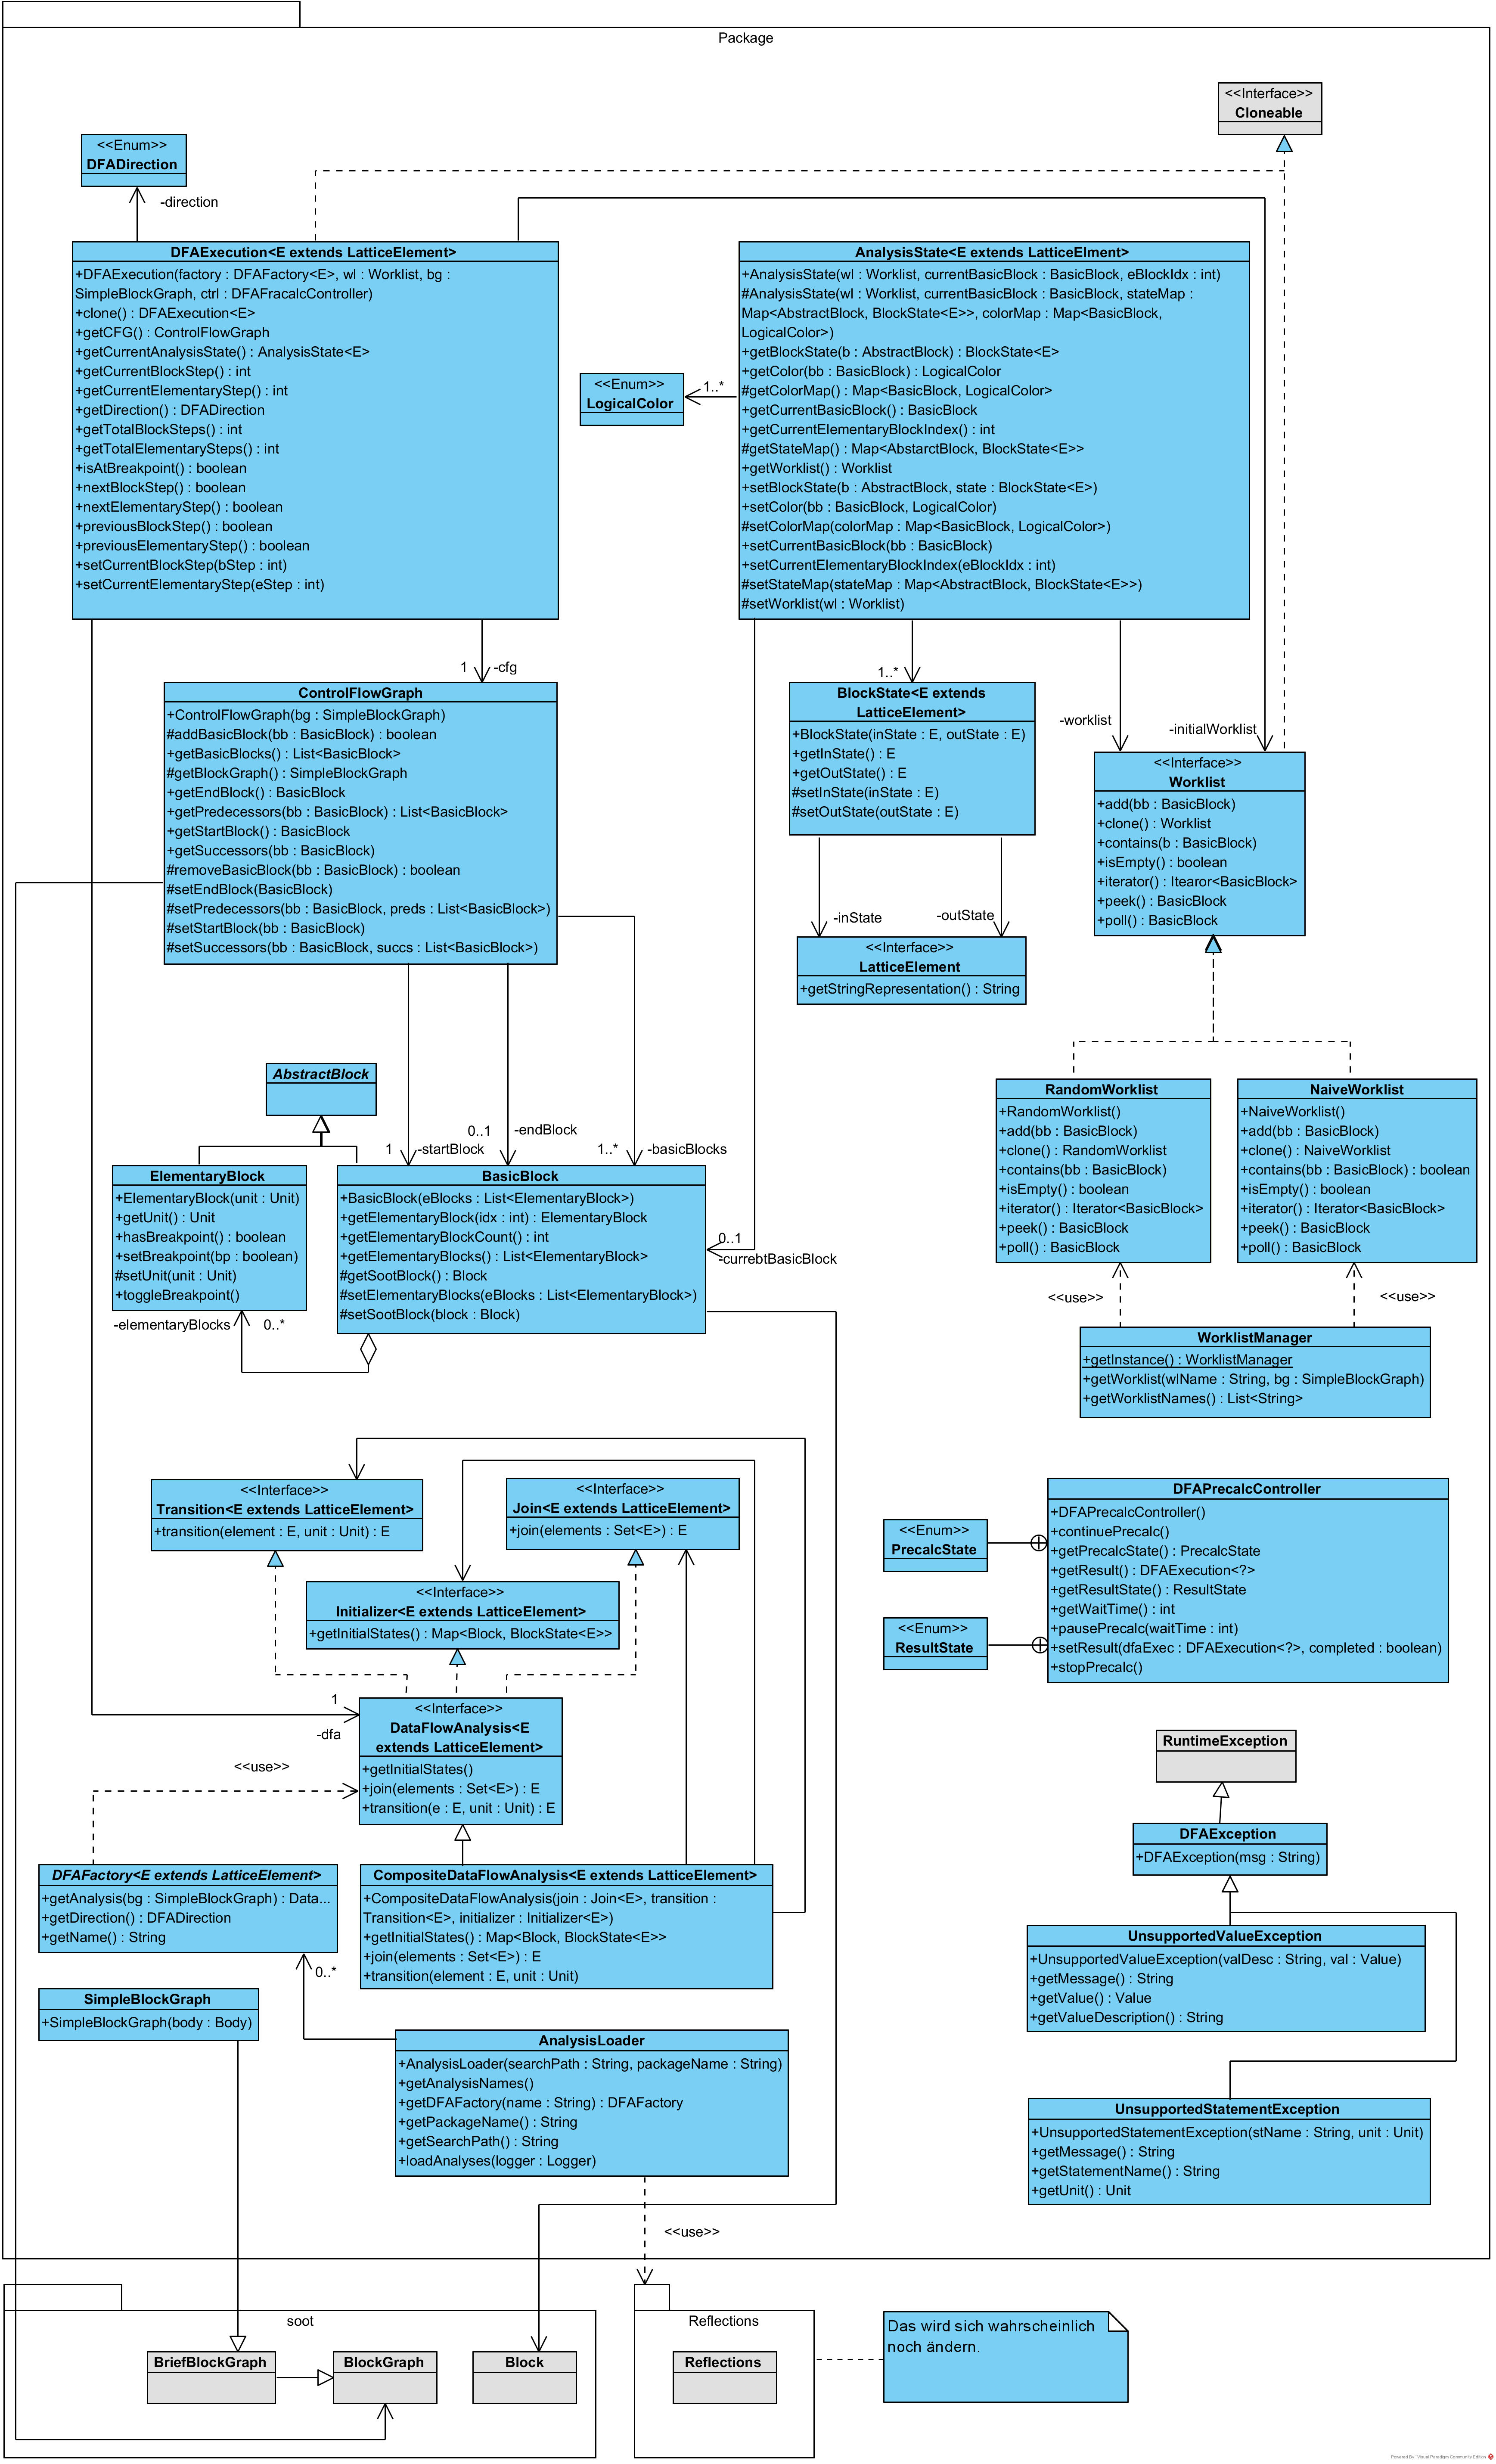
\includegraphics[width=1.0\textwidth]{Aenderungen/Klassendiagramme/DFAFramework_Impl.png}
\end{figure}

\section{Analyses}
Es wurde die Klasse \inlinecode{LocalMapElement<V>} hinzugefügt.
Diese erbt von \inlinecode{LatticeElement} und modelliert ein \inlinecode{LatticeElement}, bei dem jeder \inlinecode{JimpleLocal} ein Wert (vom Typ \inlinecode{V}) zugeordnet wird.
Dazu gibt es die Methoden \inlinecode{setValue(l:JimpleLocal,val:V)} sowie \inlinecode{getValue(l:JimpleLocal):V}.
Weiter gibt es die Methode \inlinecode{getLocalMap():Map<JimpleLocal,V>}, um Zugang zur internen \inlinecode{Map} zu ermöglichen.
Schließlich gibt es eine Standard-Implementierung von \inlinecode{getStringRepresentation():String}.
Die Klassen \inlinecode{ConstantBitsElement}, \inlinecode{ConstantFoldingElement}, \inlinecode{ReachingDefinitionsElement} und \inlinecode{TaintElement} erben nun von \inlinecode{LocalMapElement}, statt direkt von \inlinecode{LatticeElement}.

Weiter gibt es die abstrakte Klasse \inlinecode{LocalMapElementJoinHelper}\inlinecode{<V, E extends LocalMapElement<V>>}.
Diese stellt die Methode \inlinecode{performJoin(Set<E>)} bereit, die einen Join ausführt.
Dazu muss allerdings die abstrakte Methode \inlinecode{doValueJoin(elements:Set<E>,}\inlinecode{l:JimpleLocal):V} implementiert werden, die lediglich einen Join auf einzelnen Werten ausführt (denen für die angegebene \inlinecode{JimpleLocal}).

Eine weitere neue Klasse ist \inlinecode{LocalComparator}, der eine Ordnung auf \inlinecode{JimpleLocal}s festlegt. Dieser wird von \inlinecode{LocalMapElement} (und Unterklassen) benötigt, um eine konsistente Reihenfolge der \inlinecode{JimpleLocals} bei der Ausgabe zu gewährleisten.

\begin{figure}[H]
	\caption{Aktuelles Klassendiagramm für das Analyses Modul}
	\centering
	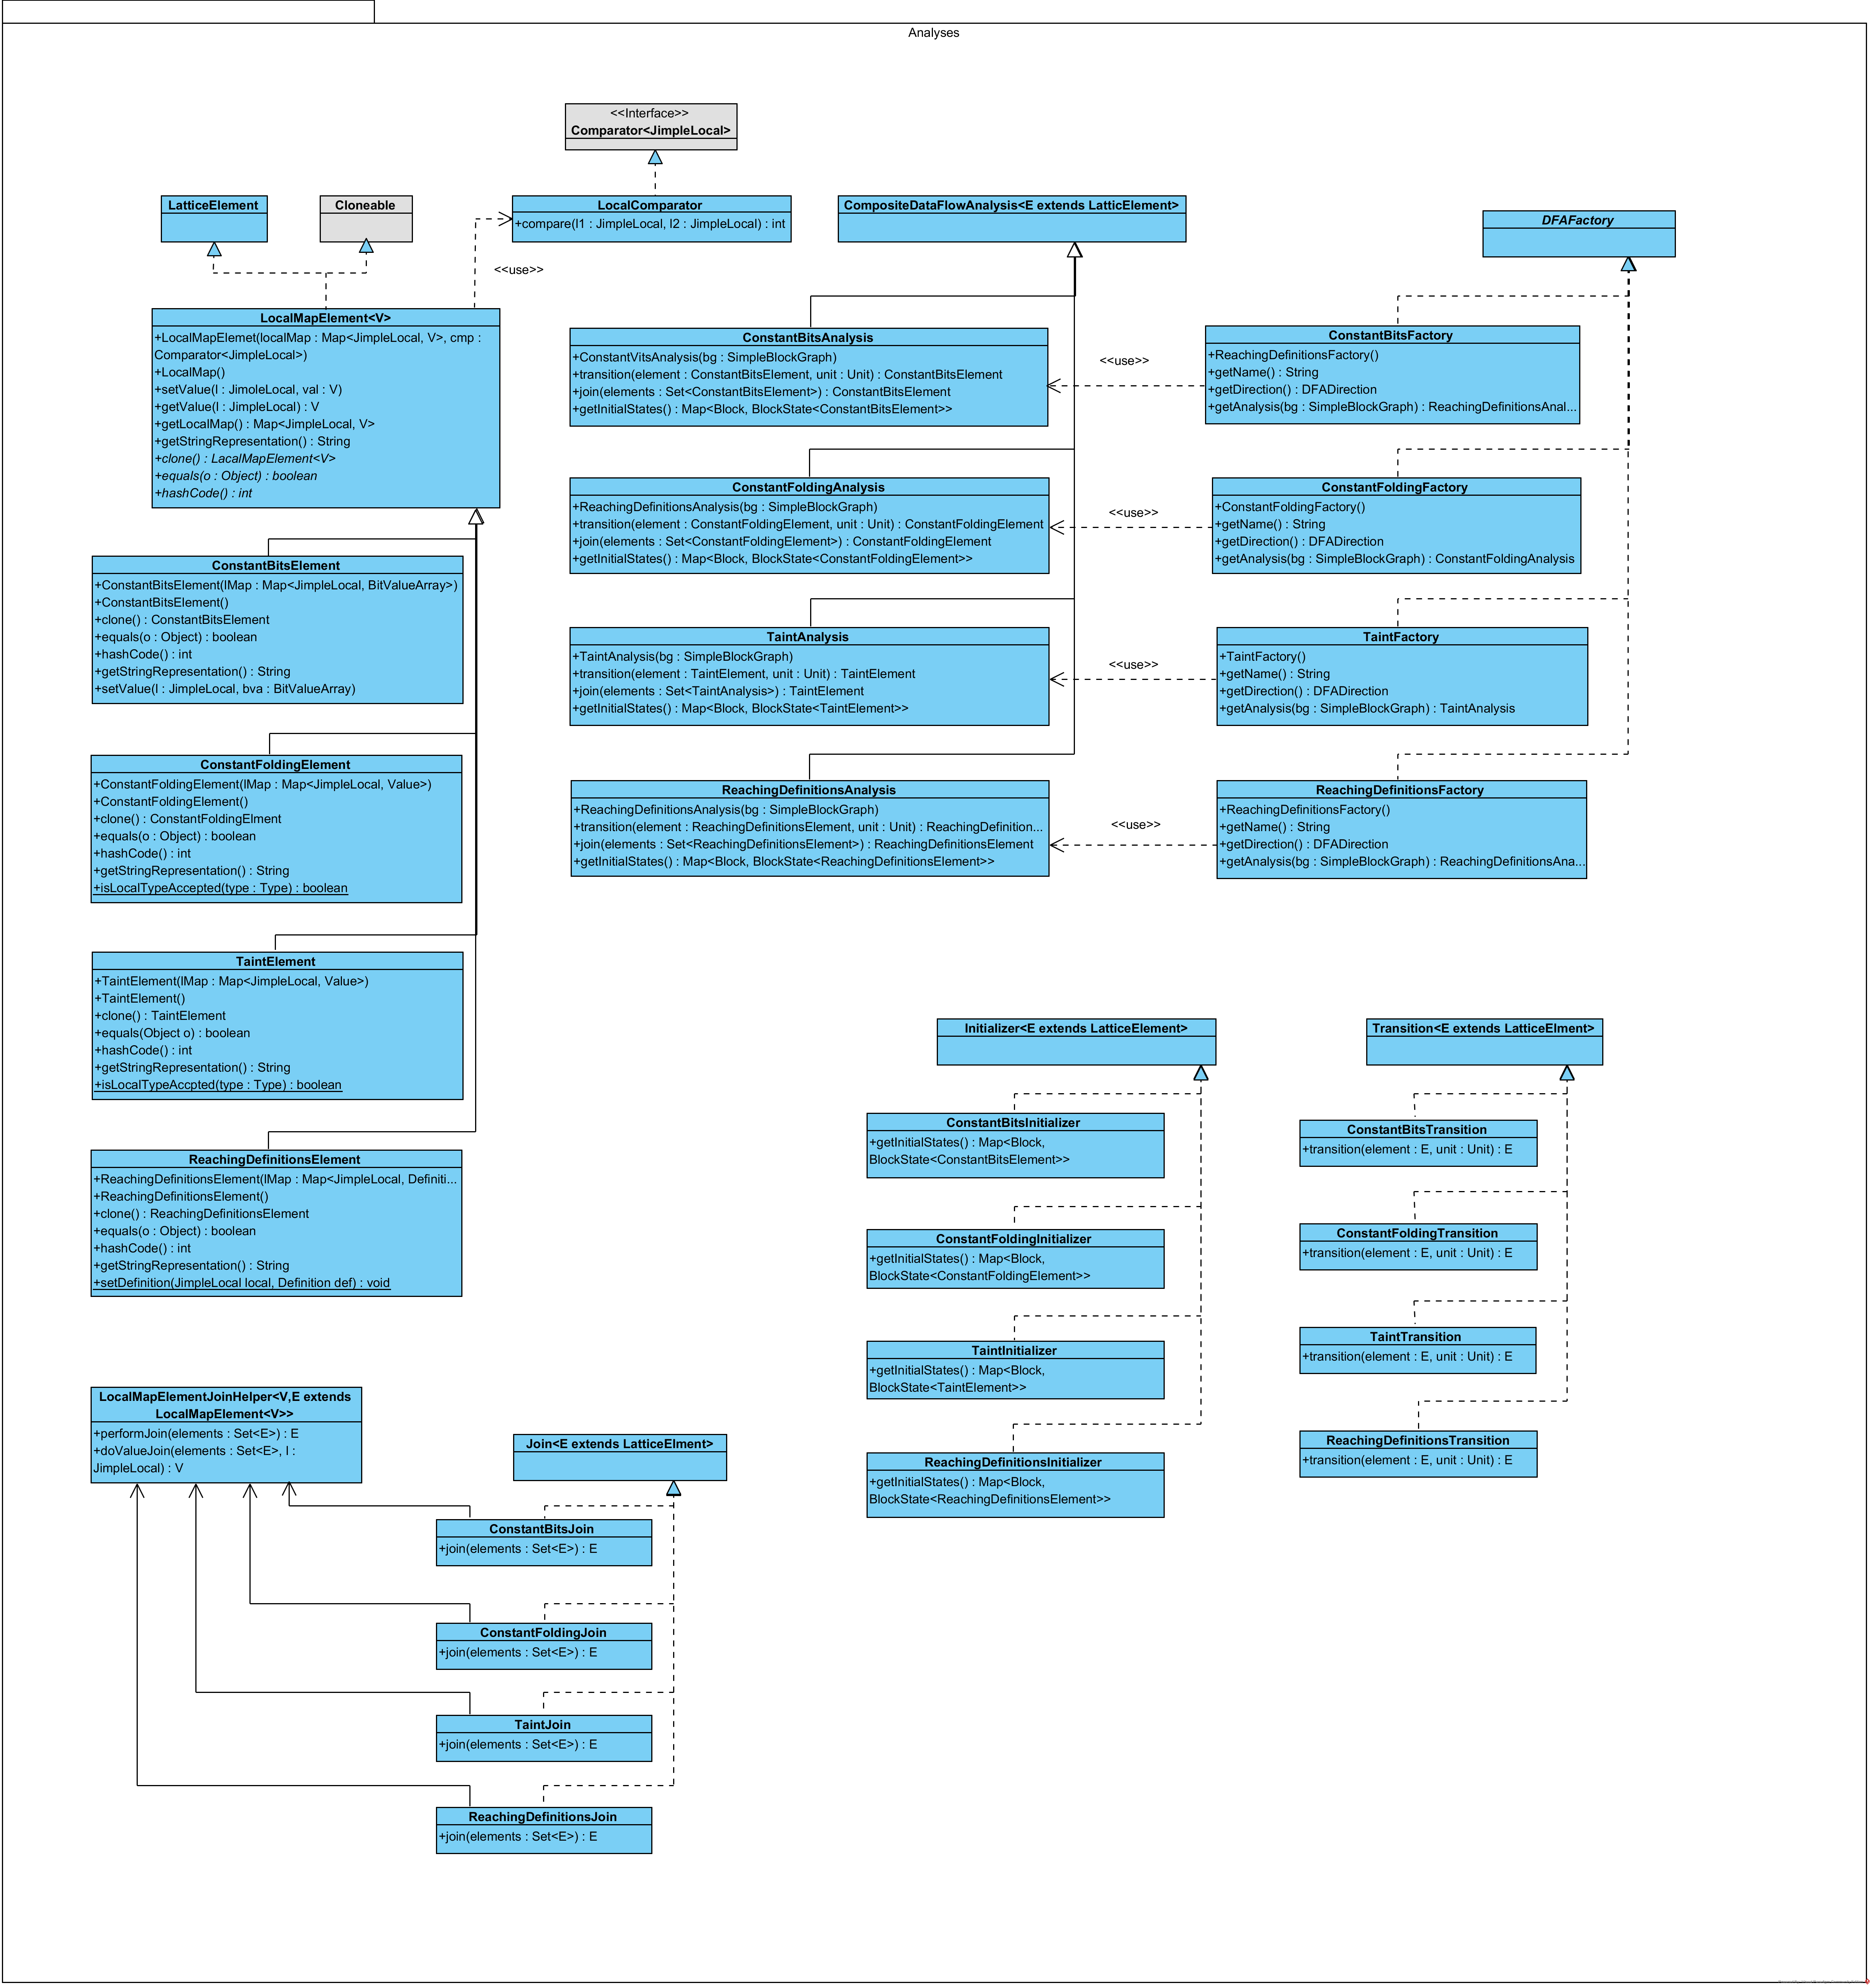
\includegraphics[width=1.0\textwidth]{Aenderungen/Klassendiagramme/Analyses_Impl.png}
\end{figure}

\newpage
\section{GUI}

\subsection{Hinzugefügte Klassen}


Das GUI-Package hat 11 neue Klassen gegenüber dem Entwurf aufzuweisen. 10 davon sind reine \enquote{Utility}-Klassen und \inlinecode{Enum}-Klassen für Konstanten.

\begin{itemize}
	\item \textbf{Colors:}
Ein \inlinecode{Enum}, welches Konstanten für die Farben der Benutzeroberfläche beinhaltet.

	\item \textbf{ControlPanelState:} Ein \inlinecode{Enum}, welches die möglichen Zustände des \inlinecode{ControlPanel} beinhaltet.

	\item \textbf{Option:} Ein \inlinecode{Enum}, welches bei Dialogen mit verschiedenen Optionen die vom Benutzer ausgewählte Option repräsentiert.

	\item \textbf{Quality:} Ein \inlinecode{Enum}, welches die ausgewählte Qualität in der \inlinecode{GraphExportBox} repräsentiert.

	\item \textbf{IconLoader:} Eine \enquote{Utility}-Klasse, welche eine statische Methode zur Verfügung stellt, um Bilder für die Benutzeroberfläche in das Programm zu laden und zu skalieren.

	\item \textbf{JComponentDecorator:} Eine \enquote{Utility}-Klasse, welche auf \inlinecode{JComponent}s Standardwerte setzt, damit diese nicht für jede Komponente einzeln gesetzt werden müssen. Dies reduziert Codeverdopplung.

	\item \textbf{JButtonDecorator:} Eine \enquote{Utility}-Klasse, welche einen \inlinecode{JButton} zuerst dem \inlinecode{JComponentDecorator} übergibt und dann selbst Standardwerte für \inlinecode{JButton}s setzt.

	\item \textbf{JLabelDecorator:} Eine \enquote{Utility}-Klasse, welche ein \inlinecode{JLabel} zuerst dem \inlinecode{JComponentDecorator} übergibt und dann Standardwerte für \inlinecode{JLabel}s setzt.

	\item \textbf{JSliderDecorator:} Eine \enquote{Utility}-Klasse, welche einen \inlinecode{JSlider} zuerst dem \inlinecode{JComponentDecorator} übergibt und dann Standardwerte für \inlinecode{JSlider} setzt.

	\item \textbf{GridBagConstraintFactory:} Eine \enquote{Utility}-Klasse, welche Standard-\inlinecode{GridBagConstraints} für eine \inlinecode{Swing}-Komponente erstellt. Diese bestimmen Platz und Größe einer Komponente im \inlinecode{GridBagLayout}.

\end{itemize}

Außerdem hat eine Komponente mehr Funktionalität gebraucht, als im Entwurf veranschlagt war. Diese ist das \inlinecode{CodeField}.
Im Entwurf war eine einfache \inlinecode{JTextArea} vorgesehen, jetzt ist das \inlinecode{CodeField} eine Klasse die von \inlinecode{JScrollPane} erbt und zwei \inlinecode{JTextArea}s beinhaltet.

\newpage
\subsection{Hinzugefügte Methoden}


Einige Klassen haben neue Funktionalität hinzugefügt bekommen.

\begin{itemize}

	\item \textbf{public File getCompilerPath():} In der \inlinecode{ProgramFrame}-Klasse. Der Benutzer muss beim ersten Starten des Programms den Pfad zu seiner \inlinecode{JDK} angeben, damit sein Programm-Code kompiliert werden kann. Dieser Pfad kann vom \inlinecode{Controller} hier abgefragt werden.

	\item \textbf{public void setCode(String code):} In der \inlinecode{InputPanel}-Klasse.
Übergibt einen \inlinecode{String} an das \inlinecode{CodeField}.

	\item \textbf{public void reset():} In der \inlinecode{StatePanelOpen}-Klasse. Setzt den Inhalt dieses \inlinecode{JPanel}s auf den Ausgangszustand zurück.

	\item \textbf{public Option getOption():} In der \inlinecode{MethodSelectionBox} und der \inlinecode{GraphExportBox}. Hierüber kann die ausgewählte Option des Benutzers abgefragt werden.

\end{itemize}

\subsection{Geänderte Klassen}


Zwei Klassen wurden umbenannt und eine dieser Klassen hat eine leicht andere Funktion.

\begin{itemize}
	\item \textbf{WarningBox:} wurde in \inlinecode{OptionBox} umbenannt und hat nun drei statt zwei \inlinecode{JButtons} zum Auswählen.

	\item \textbf{AlertBox:} wurde in \inlinecode{MessageBox} umbenannt.
\end{itemize}

\newpage 
\section{CodeProcessor}

\subsection{Geänderte Klassen}

\begin{itemize}
	\item \textbf{<<Interface>> Filter:} wurde zu \textbf{class Filter} geändert, da diese Oberklasse dafür sorgt, dass die Methoden, die manuell für die Taint-Analyse hinzugefügt wurden, herausgefiltert werden, egal welcher abgeleitete Filter verwendet wird.
\end{itemize}

\subsection{Hinzugefügte Methoden}

\begin{itemize}
	\item \textbf{public boolean filterTaint(SootMethod method):} In der \inlinecode{Filter}-Klasse. Diese Methode filtert die für die Taint-Analyse manuell hinzugefügten Methoden heraus, damit sie dem Benutzer nicht angezeigt werden.
\end{itemize}

\subsection{Geänderte Methoden}

\begin{itemize}
	\item \textbf{public String getPackageName():} in der \inlinecode{CodeProcessor}-Klasse wurde in \textbf{public String getPath():} umbenannt, da diese Methode den absoluten Pfad zu der gespeicherten .class-Datei zurück gibt.

	\item \textbf{public BlockGraph buildGraph(String methodSignature):} in der \inlinecode{GraphBuilder}-Klasse wurde zu \textbf{public SimpleBlockGraph buildGraph(String methodSignature):} geändert, da ein \inlinecode{SimpleBlockGraph} genauere Voraussetzungen spezifiziert.

	\item \textbf{public boolean filter(String methodSignature):} in der \inlinecode{Filter}-Klasse wurde zu \textbf{public boolean filter(SootMethod method):} geändert, da man mit Hilfe von Soot herausfinden kann, ob eine \inlinecode{SootMethod} eine Standard Java Methode ist oder nicht. Diese Methode wird von den abgeleiteten Klassen \inlinecode{NoFilter} und \inlinecode{StandardFilter} implementiert.
\end{itemize}

\subsection{Entfernte Methoden}

\begin{itemize}
	\item \textbf{public String getBinaries():} In der \inlinecode{CodeProcessor}-Klasse. Da diese Klasse die generierte .class-Datei lokal beim Benutzer speichert, wird diese Methode nicht mehr benötigt.
\end{itemize}


\section{Controller}

\subsection{Hinzugefügte Klasse}

\begin{itemize}
	\item \textbf{App:} In dieser Klasse befindet sich die main-Methode, welche beim Programmstart ausgeführt wird. Sie erstellt einen \inlinecode{Controller} und ein \inlinecode{ProgramFrame} und setzt für die Funktionalität des Programms wichtige Einstellungen.
\end{itemize}

\subsection{Hinzugefügte Methoden}

\begin{itemize}
	\item \textbf{public void completedAnalysis():} In der Klasse \inlinecode{Controller}. Diese Methode wird ausgeführt, nachdem die Vorberechnung der Analyse beendet wurde. Sie setzt die \inlinecode{DFAExecution}, Einstellung am \inlinecode{ControlPanel} und startet den Aufbau eines CFG im \inlinecode{GraphUIController}.

	\item \textbf{public void createExceptionBox(String message):} In der Klasse \inlinecode{Controller}. Diese Methode wird vom \inlinecode{DFAPrecalculator} aufgerufen, wenn während der Berechnung der Analyse eine Exception auftritt. Nähere Informationen zu dieser Exception werden dem Bentuzer in einer \inlinecode{MessageBox} ausgegeben.

	\item \textbf{public int getDelay():} In der Klasse \inlinecode{Controller}. Diese Methode gibt das aktuell im \inlinecode{ControlPanel} ausgewählte Delay zurück. Damit kann dieser Wert auch während der automatischen Wiedergabe der Analyseschritte geändert werden.

	\item \textbf{public List<String> getWorklist():} In der Klasse \inlinecode{Controller}. Diese Methode gibt eine Liste aller verfügbarer \inlinecode{Worklist}s aus. Diese werden in der GUI dargestellt.

	\item \textbf{public void pathSelection():} In der Klasse \inlinecode{Controller}. Diese Methode wird direkt bei Programmstart ausgeführt. Sie sorgt dafür, dass der Benutzer nach dem Pfad seiner JDK gefragt wird, falls dieser noch nicht in der Konfigurationsdatei gespeichert ist.

	\item \textbf{public void setDefaultCode():} In der Klasse \inlinecode{Controller}. Diese Methode sorgt dafür, das ein Beispielcode im Editor bei Programmstart dargestellt wird, mit welchem eine erste Analyse durchgeführt werden kann.

	\item \textbf{public boolean shouldContinue():} In der Klasse \inlinecode{Controller}. Diese Methode wird während der automatischen Wiedergabe mehrmals aufgerufen. Sie bestimmt ob diese weiter ausgeführt oder abgebrochen wird, falls ein Breakpoint erreicht wurde oder der Benutzer auf Pause geklickt hat.

	\item \textbf{protected void visibilityInput(),}\textbf{protected void visibilityWorking(,)}\textbf{protected void visiblityPlaying(),}\textbf{protected void visibilityPrecalculating():} In der Klasse \inlinecode{Controller}. Diese Methoden setzten die Sichtbarkeit und Modifizierbarkeit der unterschiedliche Panels der GUI, in Abhängigkeit vom aktuellen Zustand des Programms.
\end{itemize}

\newpage
\subsection{Geänderte Methoden}

\begin{itemize}
	\item \textbf{public void DFAPrecalculator(DataFlowAnalysis dfa, Worklist w, Blockgraph bg):} In der \inlinecode{DFAPrecalculator}-Klasse wurde in \textbf{public void DFAPrecalculator(DFAFactory<? extends LatticeElement> dfa, Worklist w, }\textbf{SimpleBlockGraph simpleBg, DFAPrecalcController precalcController, Controller controller):} geändert. Diese Änderungen ergeben sich durch die Entwurfsänderung des Packages DFAFramework.
\end{itemize}


\subsection{Entfernte Methoden}

\begin{itemize}
	\item \textbf{public DFAExecution getDFAExecution():} In der \inlinecode{DFAPrecalculator}-Klasse. Durch die hinzugefügte Klasse \inlinecode{DFAPrecalcController}, mit deren Instanz eine \inlinecode{DFAExecution} erhalten werden kann, wird diese Methode nicht mehr benötigt.
\end{itemize}

\newpage
\section{Visual Graph}

\subsection{Hinzugefügte Klassen}

Es wurde die Klasse \inlinecode{RestrictedMxGraph} hinzugefügt. Diese erbt direkt von der JGraphX-Klasse \inlinecode{mxGraph} und setzt automatisch einige Attribute des Graphen.
Dazu gehören sowohl visuelle als auch funktionale Attribute. Insbesondere wird die Erstellung von neuen Kanten durch den Benutzer unterbunden und die Verschiebung von Zeilenblöcken und Kanten deaktiviert.

\subsection{Entfernte Klassen}

Die Klasse \inlinecode{GraphListener} wurde entfernt.
Ursprünglich war geplant, jede \inlinecode{mxCell} mit einem eigenen Listener-Objekt auszustatten.
Dies wurde durch die maßgeblich simplere Implementierung ersetzt, welche einmalig einen anonymen \inlinecode{mxIEventListener} für den gesamten Graphen setzt.
Bei einer Änderung der Block- oder Zeilenauswahl wird an diesen ein \inlinecode{mxEventObject} übergeben, welches alle nötigen Informationen zur ausgewählten mxCell enthält.

\subsection{Hinzugefügte Methoden}

\subsubsection{GraphUIController}
\begin{itemize}
  \item \textbf{public void setStatePanel(StatePanelOpen statePanel)}: Diese Methode ist notwendig, damit der \inlinecode{GraphUIController} nach Änderung der Block- oder Zeilenauswahl das \inlinecode{StatePanelOpen} aktualisieren kann.
\end{itemize}

\subsubsection{UIAbstractBlock}
\begin{itemize}
  \item \textbf{abstract public AbstractBlock getDFABlock()}: Gibt den diesem Block entsprechenden Block aus dem DFAFramework zurück. Dies wird benötigt, um den zugehörigen \inlinecode{BlockState} ermitteln zu können.

  \item \textbf{abstract public String getText()}: Gibt den Text des Blocks zurück (je nach Unterklasse eine Zeile oder alle Zeilen). Dies wird benötigt, um den so erhaltenen Text im \inlinecode{StatePanelOpen} anzeigen zu können.

  \item \textbf{abstract public int[] getBlockAndLineNumbers()}: Gibt ein Array der Form [<Blocknummer>, <Zeilennummer>] zurück. Dies wird ebenfalls zur Informationsanzeige im \inlinecode{StatePanelOpen} verwendet.

  \item \textbf{public void setBlockNumber(int blockNumber)}: Wird benutzt, um die Block- bzw. Zeilennummer zu setzen. Dies geschieht im \inlinecode{GraphUIController}.
\end{itemize}

\subsubsection{UIBasicBlock}
\begin{itemize}
  \item \textbf{public void renderChildren()}: Ruft \inlinecode{render()} auf allen eingefügten Zeilenblöcken auf. Ursprünglich sollte diese Methode privat sein und von der \inlinecode{render()}-Methode dieses Blocks aufgerufen werden. Dies erwies sich wegen des Auto-Layouts als problematisch, da dieses angewendet werden muss, bevor die Zeilenblöcke eingefügt werden.
\end{itemize}

\subsubsection{UILineBlock}
\begin{itemize}
  \item \textbf{protected void setBlockMap(Map<AbstractBlock, UIAbstractBlock> map)}: Stellt dem Panel ein Block-Mapping zur Verfügung, um in der Jump-to-Action-Funktion mit Hilfe des aktuellen Blocks des DFAFrameworks den entsprechenden visuellen Block als ausgewählt markieren zu können. Dies wird vom \inlinecode{GraphUIController} durchgeführt.
  \item \textbf{public mxGraphComponent getGraphComponent()}: Diese Methode wird vom \inlinecode{GraphUIController} benötigt, um \inlinecode{UILineBlock}s zu erstellen.
  \item \textbf{public void setParentFrame(Frame frame)}: Dies wird benötigt, um den modalen Graph-Export-Dialog korrekt anzeigen zu können.
  \item \textbf{public void setJumpToAction(boolean enabled)}: Wird benötigt, um im Graph-Export die Jump-to-Action-Funktion programmatisch zu aktivieren.
\end{itemize}

\subsection{Geänderte Methoden}

\subsubsection{GraphExporter}

\begin{itemize}
  \item \textbf{exportCurrentGraph(mxGraph graph, double scale, UIAbstractBlock selectedBlock, BlockState state)}: Nimmt nun kein \inlinecode{StatePanelOpen} mehr entgegen, sondern stattdessen direkt den ausgewählten Block sowie dessen Zustand.
  \item \textbf{batchExport(DFAExecution dfa, double scale, boolean includeLineSteps)}: Nimmt nun analog zu \inlinecode{exportCurrentGraph()} einen \inlinecode{scale}-Parameter entgegen.
\end{itemize}

\subsubsection{UIBasicBlock}

Der Konstruktor nimmt zusätzlich ein \inlinecode{mxGraph}-Objekt, das zum Rendern benötigt wird, und eine \inlinecode{DFAExecution} entgegen.
Letztere ist notwendig, um die Farbe des Blocks korrekt setzen zu können.

\subsubsection{UIEdge}

Analog zum \inlinecode{UIBasicBlock} wird hier ebenfalls ein \inlinecode{mxGraph}-Objekt im Konstruktor übergeben.

\subsubsection{UILineBlock}

Auch hier wird ein \inlinecode{mxGraph}-Objekt im Konstruktor übergeben.
Zusätzlich wird auch das zugehörige \inlinecode{mxGraphComponent}-Objekt übergeben, um einen \inlinecode{MouseListener} für Breakpoints setzen zu können und den Zeilencode bei Überlänge korrekt, abhängig von der systemspezifischen Zeichenbreite, abschneiden zu können.

\subsubsection{VisualGraphPanel}

\begin{itemize}
  \item \textbf{public void renderGraph(final DFAExecution dfa, boolean isFirstRender)}: Beide Parameter wurden neu hinzugefügt. \inlinecode{dfa} wird für den Graph-Export benötigt, während \inlinecode{isFirstRender} festlegt, ob das Auto-Layout aufgerufen und der Graph sichtbar gemacht werden soll.
  \item \textbf{public mxGraph getMxGraph()}: Umbenannt (ursprünglich \inlinecode{getGraph()}).
\end{itemize}

\subsection{Entfernte Methoden}

\subsubsection{GraphUIController}

Die Methoden \inlinecode{toggleBreakpoint()}, \inlinecode{exportGraph()} und \inlinecode{toggleJumpToAction()} wurden entfernt, da entsprechende Funktionalität und Zustände ausschließlich im \inlinecode{VisualGraphPanel} von Bedeutung sind.

Weiterhin wurde \inlinecode{getVisualGraphPanel()} entfernt, da das Panel allen betreffenden Klassen bereits bekannt ist.

\subsubsection{UIAbstractBlock}

Die Methode \inlinecode{setColor()} wurde entfernt, da die Farbe nun direkt in der \inlinecode{render()}-Methode des \inlinecode{UIBasicBlock}s abgefragt wird.

\subsubsection{UILineBlock}

Die Methode \inlinecode{toggleBreakpoint()} wurde entfernt, da die entsprechende Logik ausschließlich intern in einem anonymen Listener verwendet wird.


\subsubsection{VisualGraphPanel}

Die Methode \inlinecode{showGraphExportDialog()} wurde entfernt, da diese Funktionalität ausschließlich intern verwendet wird.
